\subsection{Image Classification Setup}

Image Classification Task
    Dataset
    Architecture
    Implementation Details (coding aspect, where it is in the repo, hyperparameters)
    Evaluation
Question Answering System Task
Speech-to-Test Decoding Task




\subsubsection{Dataset}

In this paper we used EMNIST \cite{emnist} data set, which is a collection of handwritten characters and digits from NIST Special Database 19. The data is converted to 28 by 28 matrix so its format matches MNIST data set. There are six subsets in the EMNIST data set: ByClass, ByMerge, Balanced, Letters, Digits and MNIST. We chose the Letter subset because there are around 145k data in it, which will result in a decent running time without loss of information. In the Letter subset, there are 26 classes which corresponding to letter A to letter Z.
\begin{figure}[htp]
    \centering
    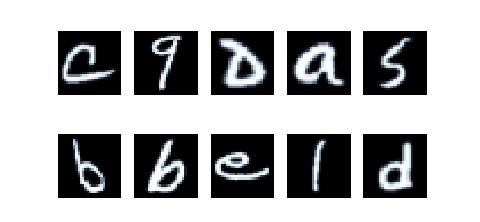
\includegraphics[width=8cm]{img/EMNIST.png}
    \caption{Data instances in EMNIST, which are handwritten 26 alphabetical characters.}
    \label{fig:EMNIST}
\end{figure}


\subsubsection{Model Architecture}
\begin{enumerate}[start=1,label={\bfseries\arabic*:}]
    \item A set of convolution layer and pooling layer to compress the image
    \item Another set of convolution layer and pooling layer to further compress the data
    \item Two fully connected layers after flattens the data to do the neural network training.
    \end{enumerate}
%The first part of the network is a straightforward CNN model and it uses Relu as activation function. It consists of two consecutive convolution layer and pooling layer in order to capture the potential features of the images. The second part of the network flattens the condensed image and then uses two fully connected layer to do the classification.

The cost function is calculated by negative log likelihood loss:
\begin{align*}
    J(y) = -log(y) 
\end{align*}
Note there is only one term in the loss function per data, which is the negative log likelihood of the predicted value of the true label. This negative loss likelihood function works better when the neural network model has a high confidence at the correct class. When training in batch, the cost function per batch is the sum of the individual negative log likelihood costs.

\subsubsection{Evaluation}



The batch size for training is {512, 1024, 2048, 4096, 8192}, the test size is 2048. we keep track of the train loss, test accuracy and test loss for every epoch when using those different optimizers to train the model. For the optimizers, we keep track of the trust ratio and the weight norm of them.


\subsection{Question Answering System Setup}

\subsubsection{Dataset}

For our QA system task, the SQuAD dataset by Rajpurkar et al. \cite{squad} is employed. There are 80,000 instances for training and 30,000 instance for testing. For each instance, there are question, answers and the context that the question and answer are based on along with the boundary label of the answer. The task is to read the question in order to (1) retrieve the relevant context and (2) then locate the start and end position of the answer. Example of such an instance is shown in Table \ref{tbl:qasystem}. 

\begin{table}[!t]
\vspace{-5pt}
\scriptsize
\vspace{7pt}
\caption{QA System SQuAD examples}\label{tbl:qasystem}
\vspace{-10pt}
\begin{center}
\begin{tabular}{ l|c|c|l}
 \multicolumn{1}{c|}{Context} &
 \multicolumn{1}{c|}{Question} &
 \multicolumn{1}{c|}{Label} &
 \multicolumn{1}{c}{Answer}\\
 %& & \\
\hline
Architecturally, the  & To whom did the Virgin  & [515,  & St Bernadette 
\\
school has a Catholic...  & Mary allegedly appear... & 541] & Soubirous \\ \hline

Architecturally, the  & What is the Grotto  & [381,  & Marian prayer 
\\
school has a Catholic...  & at Notre Dame? & 420] & \& reflection place \\ \hline

Architecturally, the  & What sits on top of the	  & [92,  & a golden statue 
\\
school has a Catholic...  & Main Building at Notre... & 126] & of the Virgin Mary \\ 

\end{tabular}
\end{center}
\vspace{-15pt}
\end{table}


\subsubsection{Implementation Details}

The first transformation for both the question and the context tokens is that they are passed through an embedding layer initialized with pre-trained GloVe word vectors. 100-dimensional vectors from 6B web crawl version are used here. There are 110K vocabularies in total. For both paragraph and question encoding, we use 2-layer bidirectional LSTMS with $h = 128$ hidden units. Our model is tested on minibatches of 64, 128, 256, and 512. 


\subsubsection{Model Architecture}


The model employed for QA end-to-end system here is called Document retriever Question Answering (DrQA) as illustrated in Figure~\ref{fig:DrQA}.  Starting from the top:
\begin{enumerate}[start=1,label={\bfseries\arabic*:}]
    \item According to Lee et al. \cite{Lee}, the questions and context can be aligned to build respective embedding of: 
    \begin{center} $f_{align} = \sum_j \alpha_{i, j} E(q_j)$. \end{center}
    
    Where $\alpha$ is single dense layer with relu non-linearity and $E()$ represents the glove embeddings. This layer help initialize what portion of the context is more important or relevant with respect to the question.
    
    \item In order to understand the representation of these glove and aligned paragraphs, these are passed to stacked bi-LSTM. LSTM is expressed as: 
    $z_t &= \sigma(W_z x_t + U_z h_{t-1} + b_z) \\
    r_t &= \sigma(W_r x_t + U_r h_{t-1} + b_r) \\
    \tilde{h}_t &= f(W_h x_t + r_t \circ U_h h_{t-1} + b_h) \\
    h_t &= (1 - z_t) h_{t-1} + z_t \tilde{h}_t
    $
    
    \item Then the importance of each word in the question is calculated through Linear Attention layer as $b$ below with $w$ as a trainable weight vector:
    \begin{center} 
    $b_j = \frac{e^{w \cdot q_j}}{\sum_{j'}e^{w\cdot q_{j'}}}$
    \end{center}
    
    \item Finally, to predict the accurate answer's span tokens, there are two bilinear classifiers to respectively predict the probabilities of start and end tokens of the span: 
    \begin{center} 
    $P_{start}(i) \propto e^{p_iW_sq}$ \\
    $P_{end}(i) \propto e^{p_iW_eq}$
    \end{center}
    
    
\end{enumerate}


\begin{figure}[!t]
    \centering
    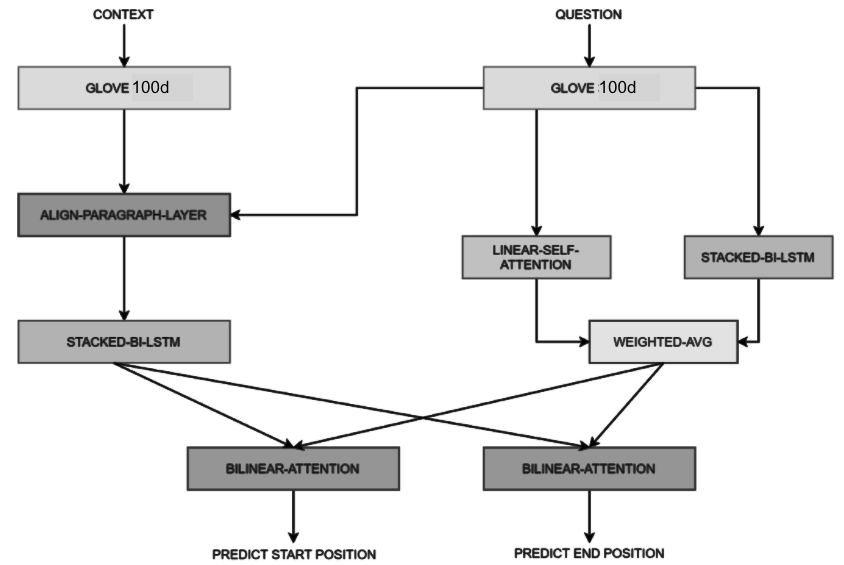
\includegraphics[width=\linewidth]{img/DrQA.png}
    \caption{Document Reader model architecture part of DrQA}
    \label{fig:DrQA}
\end{figure}

% As the name suggested, the model included Document Retriever and Document Reader: 




\subsubsection{Evaluation}

The model's loss function for updating each batch and epoch is the sum of cross entropy between the predicted and actual of the two tokens. 


\subsection{Speech-to-Text Setup}


% SpeechRecognitionModel(
%   (cnn): Conv2d(1, 32, kernel_size=(3, 3), stride=(2, 2), padding=(1, 1))
%   (rescnn_layers): Sequential(
%     (0): ResidualCNN(
%       (cnn1): Conv2d(32, 32, kernel_size=(3, 3), stride=(1, 1), padding=(1, 1))
%       (cnn2): Conv2d(32, 32, kernel_size=(3, 3), stride=(1, 1), padding=(1, 1))
%       (dropout1): Dropout(p=0.3, inplace=False)
%       (dropout2): Dropout(p=0.3, inplace=False)
%       (layer_norm1): CNNLayerNorm(
%         (layer_norm): LayerNorm((64,), eps=1e-05, elementwise_affine=True)
%       )
%       (layer_norm2): CNNLayerNorm(
%         (layer_norm): LayerNorm((64,), eps=1e-05, elementwise_affine=True)
%       )
%     )
%     (1): ResidualCNN(
%       (cnn1): Conv2d(32, 32, kernel_size=(3, 3), stride=(1, 1), padding=(1, 1))
%       (cnn2): Conv2d(32, 32, kernel_size=(3, 3), stride=(1, 1), padding=(1, 1))
%       (dropout1): Dropout(p=0.3, inplace=False)
%       (dropout2): Dropout(p=0.3, inplace=False)
%       (layer_norm1): CNNLayerNorm(
%         (layer_norm): LayerNorm((64,), eps=1e-05, elementwise_affine=True)
%       )
%       (layer_norm2): CNNLayerNorm(
%         (layer_norm): LayerNorm((64,), eps=1e-05, elementwise_affine=True)
%       )
%     )
%     (2): ResidualCNN(
%       (cnn1): Conv2d(32, 32, kernel_size=(3, 3), stride=(1, 1), padding=(1, 1))
%       (cnn2): Conv2d(32, 32, kernel_size=(3, 3), stride=(1, 1), padding=(1, 1))
%       (dropout1): Dropout(p=0.3, inplace=False)
%       (dropout2): Dropout(p=0.3, inplace=False)
%       (layer_norm1): CNNLayerNorm(
%         (layer_norm): LayerNorm((64,), eps=1e-05, elementwise_affine=True)
%       )
%       (layer_norm2): CNNLayerNorm(
%         (layer_norm): LayerNorm((64,), eps=1e-05, elementwise_affine=True)
%       )
%     )
%   )
%   (fully_connected): Linear(in_features=2048, out_features=500, bias=True)
%   (birnn_layers): Sequential(
%     (0): BidirectionalGRU(
%       (BiGRU): GRU(500, 500, batch_first=True, bidirectional=True)
%       (layer_norm): LayerNorm((500,), eps=1e-05, elementwise_affine=True)
%       (dropout): Dropout(p=0.3, inplace=False)
%     )
%     (1): BidirectionalGRU(
%       (BiGRU): GRU(1000, 500, bidirectional=True)
%       (layer_norm): LayerNorm((1000,), eps=1e-05, elementwise_affine=True)
%       (dropout): Dropout(p=0.3, inplace=False)
%     )
%     (2): BidirectionalGRU(
%       (BiGRU): GRU(1000, 500, bidirectional=True)
%       (layer_norm): LayerNorm((1000,), eps=1e-05, elementwise_affine=True)
%       (dropout): Dropout(p=0.3, inplace=False)
%     )
%   )
%   (classifier): Sequential(
%     (0): Linear(in_features=1000, out_features=500, bias=True)
%     (1): GELU()
%     (2): Dropout(p=0.3, inplace=False)
%     (3): Linear(in_features=500, out_features=29, bias=True)
%   )
% )
% image of the network is the network.png
% https://www.assemblyai.com/blog/end-to-end-speech-recognition-pytorch

\begin{figure}[!t]
    \centering
    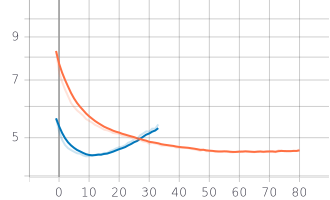
\includegraphics[width=0.7\linewidth]{img/adam_blue_lamb_orange_drqa_256.png}
    \caption{Adam (light blue) and LAMB (orange) test loss convergence graph with batch size of 256.}
    \label{fig:256}
\end{figure}

\subsubsection{Dataset}

Data was preprocessed into spectrograms at a sample rate of 16khz. The task is to map an audio spectrogram frame to one of the 29 output classes (26 alphabet characters, an apostrophe, a space, and an <END> token). 


\subsubsection{Implementation Details}

Residual CNN block includes: 3 layers with 32x32 window size, stride of 2. A fully connected layer from ResCNN to GRU-RNN with 2048 to 500 dimension. Bidirectional GRU-RNN block have three layers with 500 input feature dim and 1000 output features. A final fully connected layer with 1000 input and 500 output. Dropout of 30\%.

\subsubsection{Model Architecture}

Model is similar to Deep Speech 2, model, but first preprocesses the data into a spectrogram, then these are fed into 3 Residual CNN blocks to extract feature vectors of length 500 from the audio data, and a set of 3 bidirectional GRU-RNN layers to translate the extracted features into an intermediate output vector, which is fed into a fully connected layer, then a softmax, then a 28 long vector mapping of probabilities of corresponding letters or symbols.

\begin{figure*}[!t]
    \centering
    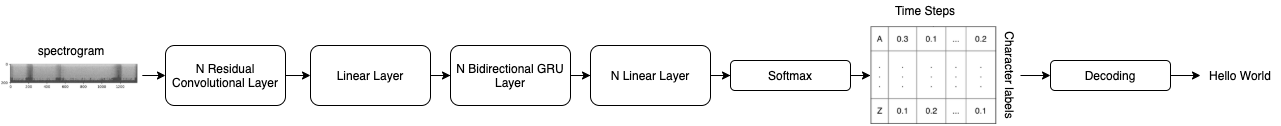
\includegraphics[width=\linewidth]{img/speech.png}
    \caption{A variant of Deep Speech 2 architecture that utilizes Res-CNN and GRU.}
    \label{fig:deepSpeech}
    \vspace{-10pt}
\end{figure*}

\begin{enumerate}[start=1,label={\bfseries\arabic*:}]
    \item Residual network consists of stacked ``residual units'' inspired by He et al. but with layer norm to learn the audio features expressed as:
    \begin{center}
    $x_{l + 1} = ReLU(h(x_l) + F(x_l, W_l))$ \\
    \end{center}
    
    \item A fully connected layer to compress the model representation before passing it over. 
    
    \item Bidirectional GRU-RNN is then utilized to leverage the features to learn the representation of the audio's spectrogram frames before the current step and after it as well. 
    
    \begin{center}
    
    $z_t &= \sigma(W_z x_t + U_z h_{t-1} + b_z)$ \\
    $r_t &= \sigma(W_r x_t + U_r h_{t-1} + b_r)$ \\
    $\tilde{h}_t &= f(W_h x_t + r_t \circ U_h h_{t-1} + b_h)$ \\
    $h_t &= (1 - z_t) h_{t-1} + z_t \tilde{h}_t$

    \end{center}
    
    $\sigma(\cdot)$ is the sigmoid function, $z$ and $r$ represent the \emph{update} and \emph{reset} gates respectively. This is slightly different from the standard GRU in that the hidden state $h_{t-1}$ is multiplied by $U_h$ prior to scaling by the reset gate. This allows for all operations on $h_{t-1}$ to be computed in a single matrix multiplication. Moreover, Amodei et al. found similar performance for $tanh$ and clipped-ReLU for nonlinear transformation so clipped-ReLU is picked for simplicity and uniformity with the rest of the network.

    
    \item A final fully connected layer takes the inputs from the feature analysis and applies weights to predict the correct label.
    
    \item A Gaussian Error Linear Unit (GELU) activation layer as: 
    
    \begin{center}
    $GELU(x) = xP(X \leq x) = x \cdot \frac{1}{2} [1 + erf(\frac{x}{\sqrt{2}}]$
    \end{center}
    
    \item A linear layer to map the results to final probabilities for each mapping of corresponding letters or symbols. 
    
\end{enumerate}



\subsubsection{Evaluation}

The model is trained on the Connectionist Temporal Classification (CTC) loss function when aligning audio to transcript, which was originated by \cite{CTC} as shown here for a single (X, Y) pair: 
\begin{center}
$p(Y | X) = \sum_{A\in A_{X, Y}} \prod_t^T = p_t(a_t |. X)$    
\end{center}

CTC first computed the probability for a single alignment step-by-step over multiple sequences then marginalizes over the set of valid alignments to get a distribution over outputs.  